\textcolor{black}{\section{Procedimiento}}

\subsection{PARTE 1}

\begin{figure}%[H]
	\centering
	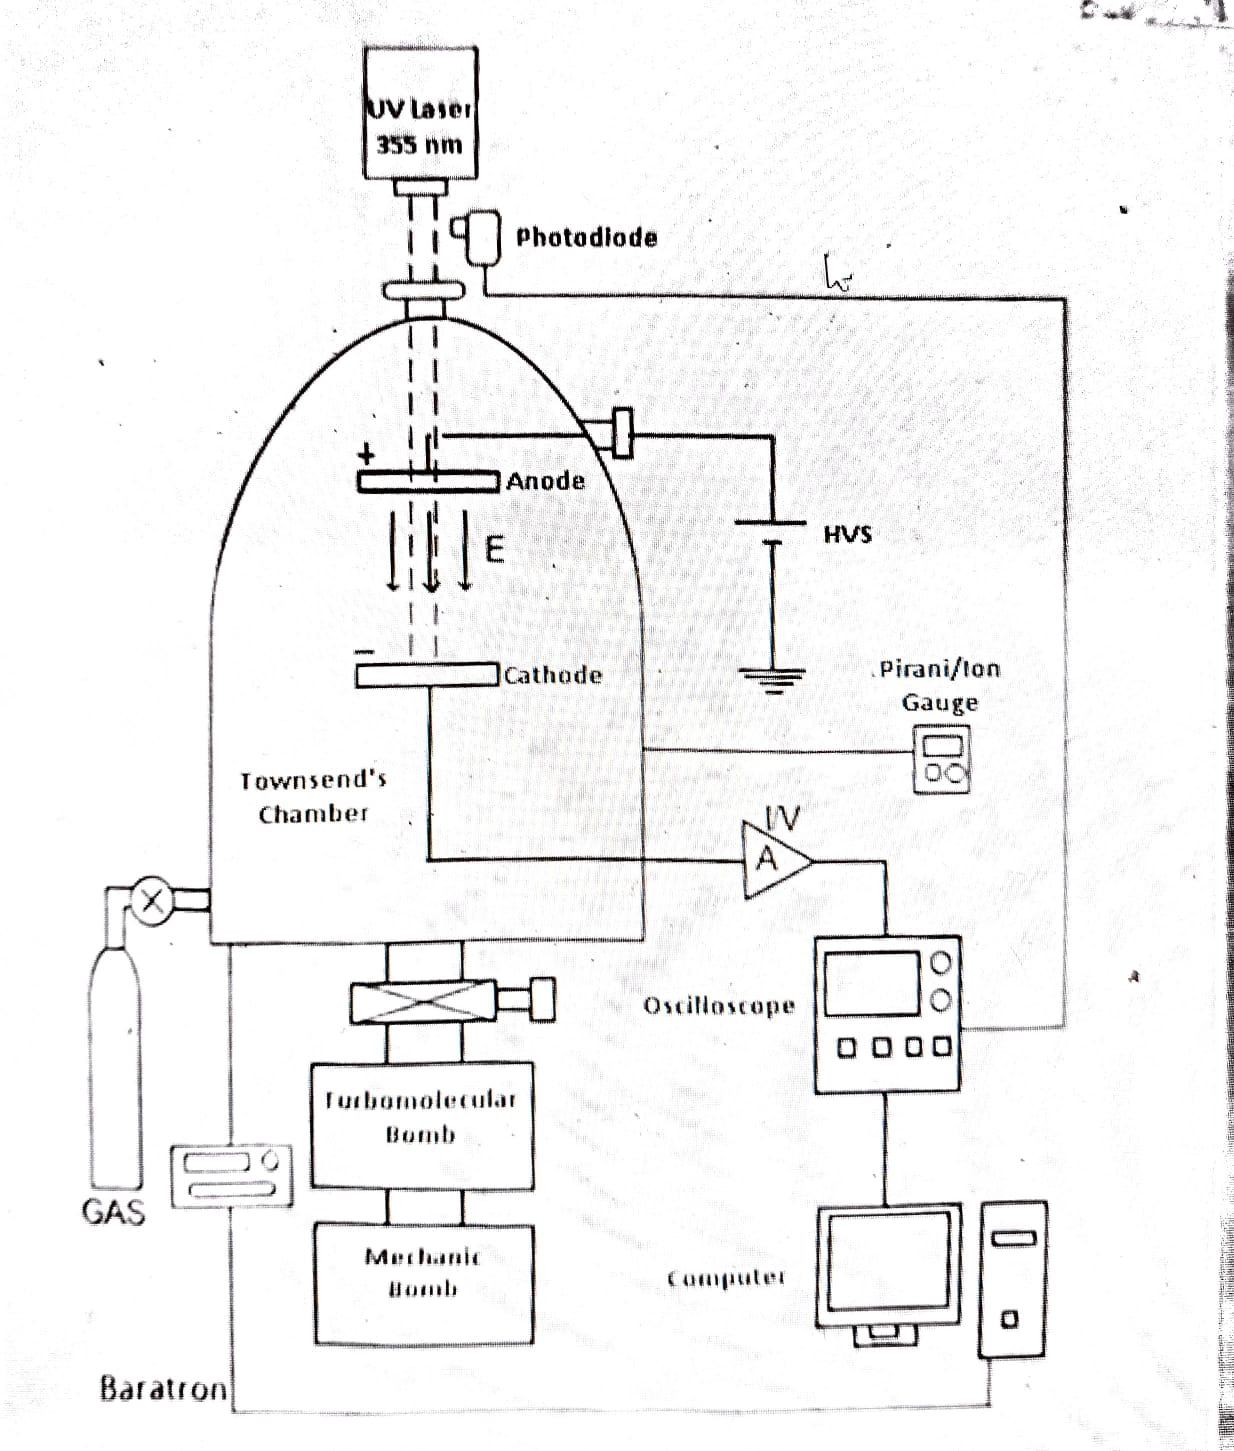
\includegraphics[scale=0.14]{figs/DiagramaTownsend.jpeg}
	\caption{Diagrama del arreglo experimental}
	\label{fig:DiagTownsend}
\end{figure}

\noindent El arreglo para poder observar el efecto Ramsauer-Townsend se muestra en la Figura \ref{fig:DiagTownsend}. Primero encendemos la bomba mecánica para extraer el aire dentro de la cámara de Townsend y así poder purgarla, después encendemos la bomba turbomolecular para poder lograr un vacío de $2.5e-6$ Torrs. Una vez teniendo el vacío, se le inyecta una mezcla de 1\% de Nitrógeno en Argón. Se inició con 200.2 Torrs, teniendo 2 Torrs de Nitrógeno con 198 Torrs de Argón.

Después encendemos el láser EKSPLA NT 342B de $\lambda = 355\,nm$, tras verificar su funcionamiento, lo disparamos hacia el cátodo. En el computador modificamos la intensidad del láser y el voltaje suministrado entre los electrodos, de tal manera que el osciloscopio no se saturara, ni generara descargas eléctricas dentro de la cámara. Se inició con un campo eléctrico reducido $\frac{E}{N} = 1\,Td$ donde, el equivalente de Townsend a Volts es $1\,Td = 158\,V$.

El osciloscopio registraba la subida y caída del voltaje en función del tiempo como se muestra en la Figura \ref{osciloscopio}. Con ayuda de los cursores del osciloscopio, se registraron los tiempos de tránsito electrónico, definidos a la mitad de la caída de voltaje.

\begin{figure}[H]
	\centering
	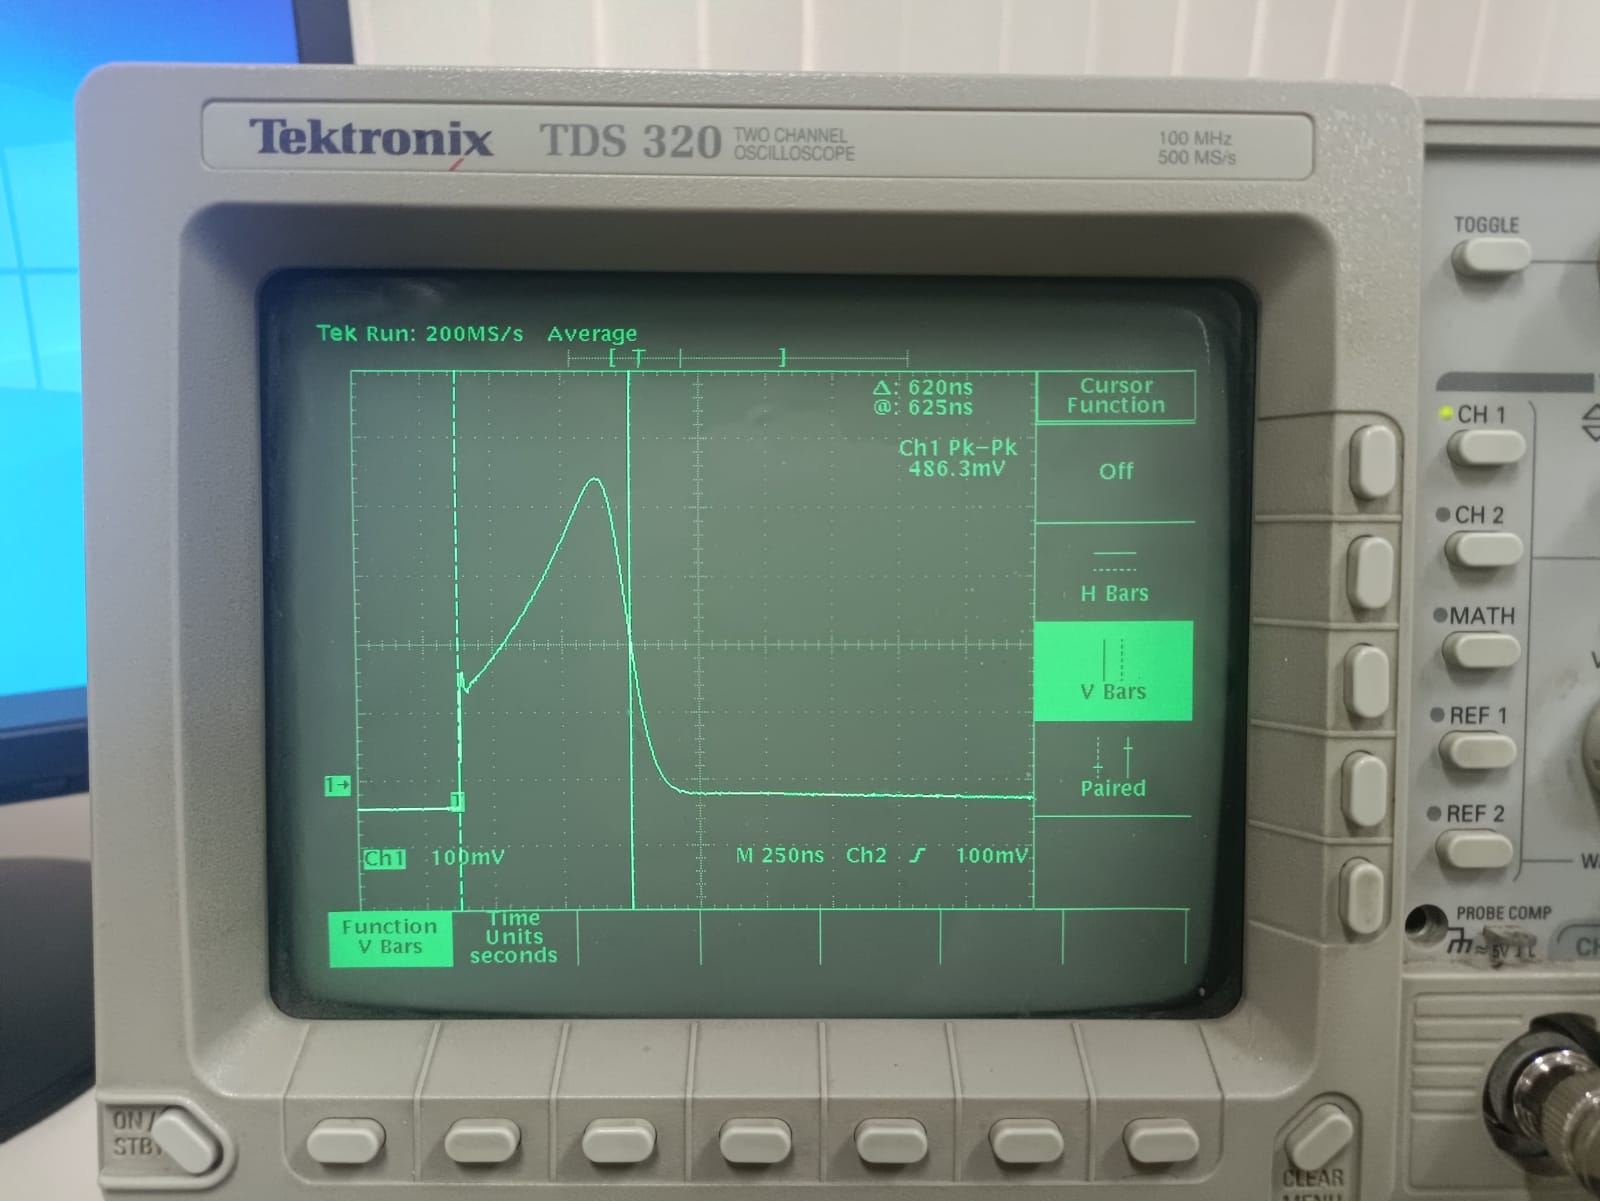
\includegraphics[scale=0.12]{figs/Osciloscopio.jpeg}
	\caption{Señal de salida mostrada en el osciloscopio, la barra vertical se ajustaba manualmente mostrando el tiempo de tránsito electrónico}
	\label{osciloscopio}
\end{figure}

Esto se hizo para una misma presión, aumentando varias veces el campo eléctrico reducido $\frac{E}{N}$ y la intensidad del láser, registrando sus tiempos de tránsito electrónico, hasta que la señal en el osciloscopio dejara de ser visible o confiable, debido al ruido.

Una vez acabado el procedimiento para esta presión, se disminuyó la cantidad de la mezcla de Nitrógeno y Argón y se volvieron a repetir las mediciones con el mismo procedimiento. Esto se hizo para presiones de:
$200.2$ Torrs, $182.0$ Torrs, $162.4$ Torrs, $142.6$ Torrs, $101.7$ Torrs, $60.8$ Torrs, $31.45$ Torrs, $10.1$ Torrs.

Los datos registrados se usaron para obtener la velocidad de deriva de las partículas, usando que $d=3\,cm$ es la separación de los electrodos. De esta manera, para cada valor del campo reducido $\frac{E}{N}$ le correspondía una velocidad de deriva $v$ las cuales se graficaron para las distintas presiones.

\subsection{PARTE 2}
\noindent Se utilizó un módulo pre-fabricado para polarizar adecuadamente los electrodos de un bulbo 2D21 (Figura \ref{Diag1}). Se utilizaron dos fuentes de alimentación UNI-T UDP6721 para polarizar al filamento y para la polarización del ánodo-cátodo; para la primera se configuró una fuente a $2\,A$ y para la segunda a $1\,A$. Se siguió el diagrama de conexión de la Figura \ref{Diag2}, utilizando también dos multímetros Steren UNI-T MUL-600.

\begin{figure}[H]
	\centering
	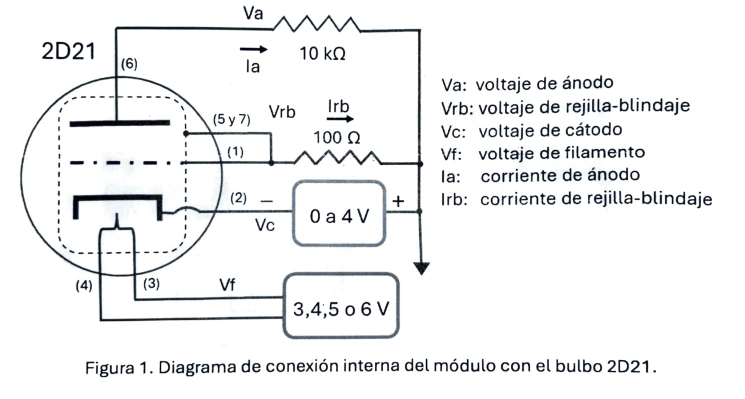
\includegraphics[scale=0.4]{figs/Diag1.png}
	\caption{Diagrama de conexión interna del módulo con el bulbo 2D21.}
	\label{Diag1}
\end{figure}

\begin{figure}%[H]
	\centering
	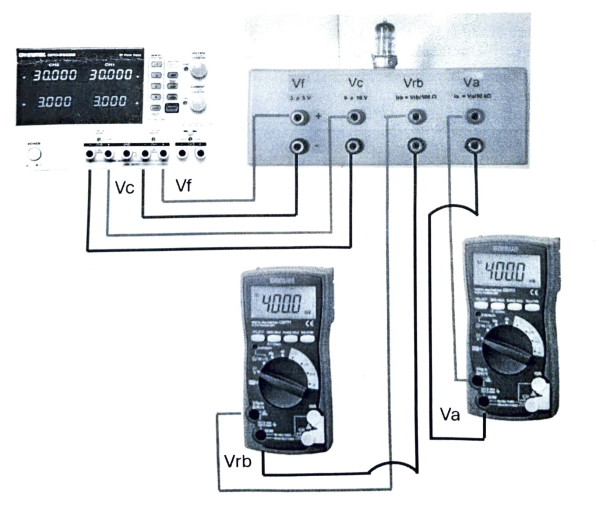
\includegraphics[scale=0.4]{figs/Diag2.png}
	\caption{Diagrama de conexión interna del módulo con el bulbo 2D21.}
	\label{Diag2}
\end{figure}

Una vez hecha las conexiones se incrementó el voltaje del filamento ($V_f$) hasta $2\,V$ y se dejó reposar durante $2$ minutos para que el filamento se calentara. Después, se varió el voltaje del cátodo ($V_c$) de $0\,V$ a $4\,V$ en pasos de $0.1\,V$ , y se tomó registro del voltaje del ánodo ($V_a$) y de la rejilla-blindaje ($V_{rb}$) a través de los multímetros. Este procedimiento se repitió para un $V_f$ de $3\,V$ y $4\,V$, y se graficaron tanto $V_{rb} \textit{ vs. } V_c$ como $V_a \textit{ vs. } V_c$ para cada uno de los tres $V_f$.

Finalmente, se hizo prueba de un software del laboratorio que automatiza el procedimiento anterior para un $V_f$ que nosotros le indiquemos, y el producto que devuelve es el registro de los voltajes $V_a$ y $V_{rb}$; así, también se hizo una comparación de los métodos de medición.